\chapter{退化预测边缘计算架构}
在第二章中的特征工程部分,我们在通过时域和频域计算特征因子的时候,使用了大量的统计特征、快速傅里叶变换等算法。这些算法需要很大的CPU计算开支,在机床数目不多的时候,单一计算机可以完成特征值与神经网络计算,但是在真实生产环境下,一个工厂通常有几十台加工中心组成,如果所有加工中心的传感器获取到的数据都由云端一台计算机进行汇总计算,这对于计算机的性能以及网络传输设备的要求很高。为解决此问题,我们采用了边缘计算的方式,将机床传感器数据的传输和计算分层,由不同设备完成。这样就可以解决设备算力和网络带宽问题。
 \par
边缘计算,是指在靠近物或数据源头的一侧,采用网络、计算、存储、应用核心能力为一体的开放平台,就近提供最近端服务。\par
简单来说,就是把计算的能力放到边缘。我们不再需要把所有的数据传到云端进行分析后反馈,而是可以赋予当地的设备或身边的传感器进行快速处理并反馈,平衡了大量数据产生时对反馈及时性的需求。\par
% 
\section{退化预测边缘计算的优势}
\subsection{低延迟}
计算能力部署在设备侧附近,设备请求实时响应,边缘计算设备可以直接获取传感器信号,并进行特征计算。
\subsection{低带宽运行}
将工作迁移至更接近于用户或是数据采集终端的能力能够降低站点带宽限制所带来的影响。尤其是当边缘节点服务减少了向中枢发送大量数据处理的请求时。
\subsection{隐私保护}
数据本地采集、本地分析、本地处理,有效减少了数据暴露在公共网络的机会,保护了数据隐私。
% \section{}
% \subsection{}
\section{边缘计算架构详解图}
\begin{figure}[htp]
    \centering
    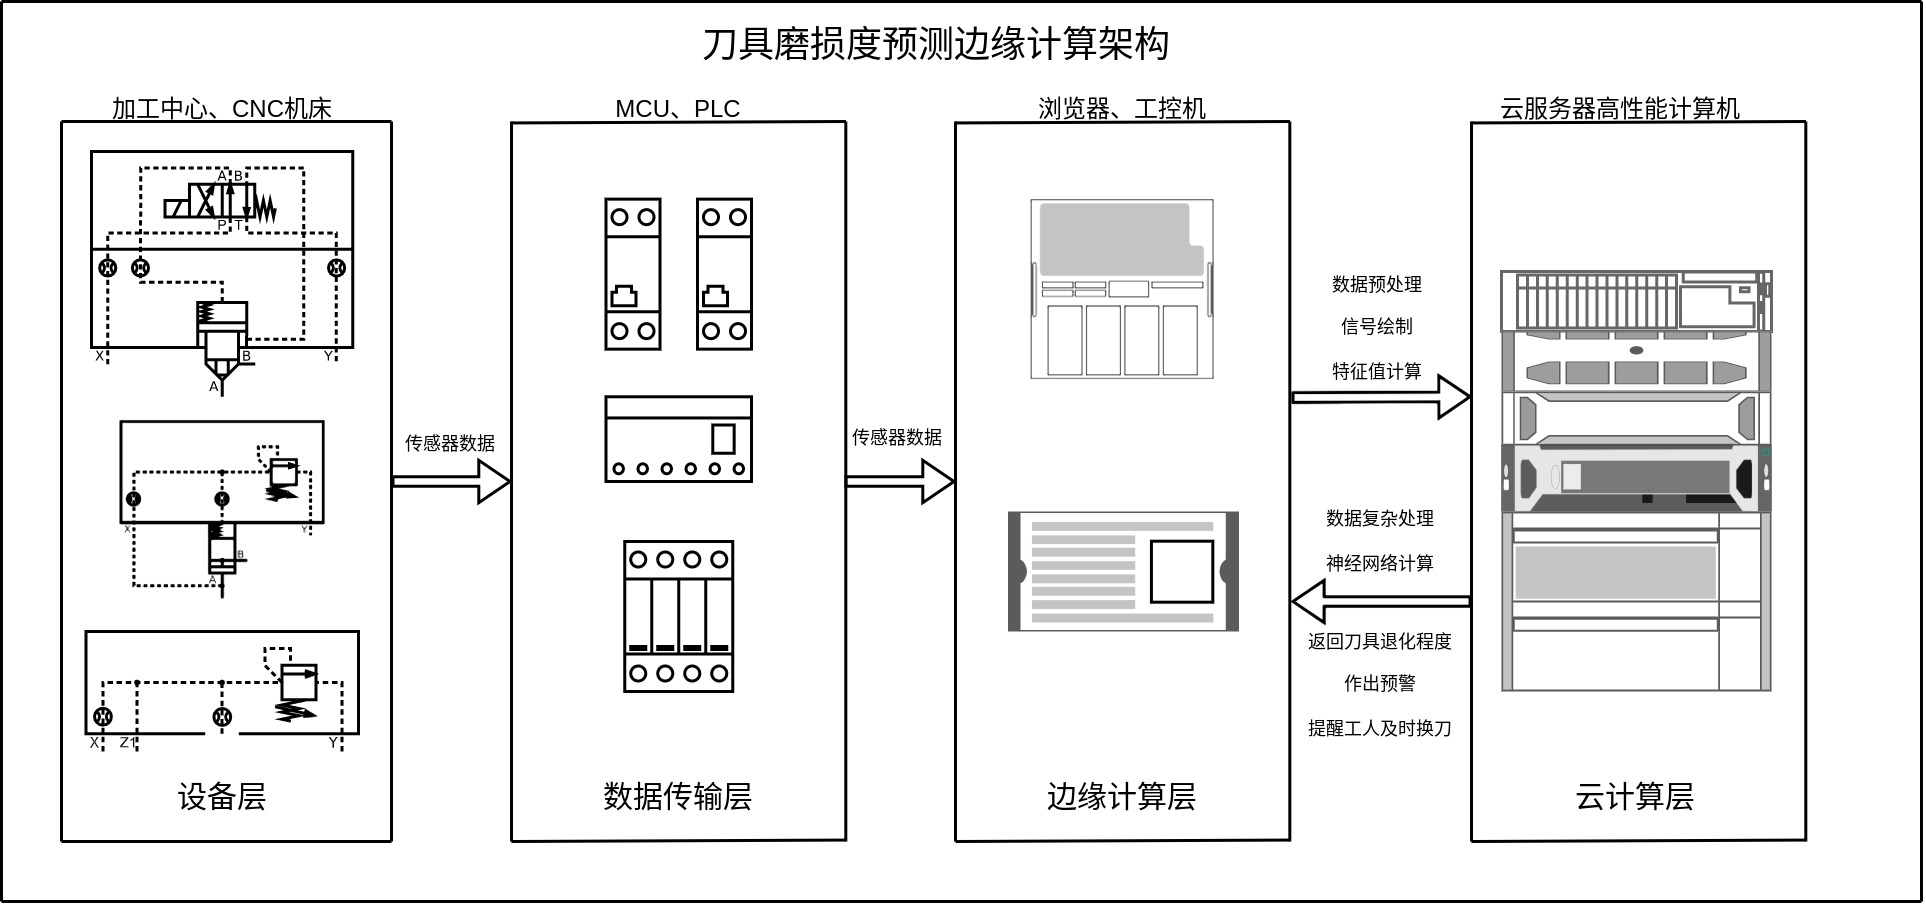
\includegraphics[width=14cm]{Chapter4/edge_compute_arch.jpg}
    \caption{刀具退化边缘计算架构}
\end{figure}
% 
% 我们设计的刀具退化预测边缘计算架构由四层组成,它们分别是:由加工中心组成的设备层(产生信号),由PLC或是单片机组成的传输层(将设备层获取到的传感器信号传递给边缘计算层),由边缘设备(工控机或是计算机浏览器等)组成的边缘计算层(负责计算信号特征值、绘制信号图像、传递特征值给云端设备以及显示云端设备返回的刀具退化程度),由云服务器或是高性能计算机组成的云计算层(将获取到的机床特征值进行神经网络计算,预测刀具退化程度并把该数据返回给边缘计算层)。\par
% \section{边缘计算实战(实验级) \\ WebAssembly实现特征值计算}
% \subsection{Web Assembly介绍}
% WebAssembly,即wasm是一个虚拟指令集体系架构(virtual ISA),整体架构包括核心的ISA定义、二进制编码、程序语义的定义与执行,以及面向不同的嵌入环境(如Web)的应用编程接口(WebAssembly API)。其初始目标是为C/C++等语言编写的程序经过编译,在确保安全和接近原生应用的运行速度更好地在Web平台上运行。 \par
% WebAssembly是一种可以使用非 JavaScript 编程语言编写代码并且能在浏览器上运行的技术方案。可以把WebAssembly 看成一种目标汇编语言,而 WebAssembly 与其他的汇编语言不一样,它不依赖于具体的物理机器。可以抽象地理解成它是概念机器的机器语言,而不是实际的物理机器的机器语言。\par
% % 
% \subsection{Web Serial API介绍}
% Web Serial API 是一套允许网站从串行设备通过脚本读取和写入的方式微控制器、3D 打印机和其他串行设备等设备进行通信的一套API。\footnote{\href{https://developer.mozilla.org/en-US/docs/Web/API/Serial}{Web Serial API是浏览器API,对于浏览器有限制,更多查看文档:https://developer.mozilla.org/en-US/docs/Web/API/Serial}} \par
% % 
% \newpage
% \subsection{单片机获取传感器信号与浏览器WASM计算特征值}
% 将单片机与机床测量电流信号的传感器、测量振动和噪声信号的传感器连接,同时单片机USB串行数据接口与电脑USB接口相连,编写电脑端Web程序实现Web Serial API连接(目前Web Serial只支持Chrome浏览器,Firefox和Edge目前不支持),运行Web页面就可以实时获取单片机从传感器获取到的信号,电脑端Web Assembly程序就可以对这些信号进行特征值计算。我们使用的WASN采用的是C语言写的算法,编译目标为*.wasm文件(C算法来自于MATLAB文件,使用MATLAB Coder将MATLAB文件编译为C代码,具体详见第五部分工业应用:模型部署)。\par
% % 
% \begin{figure}[htp]
%     \centering
%     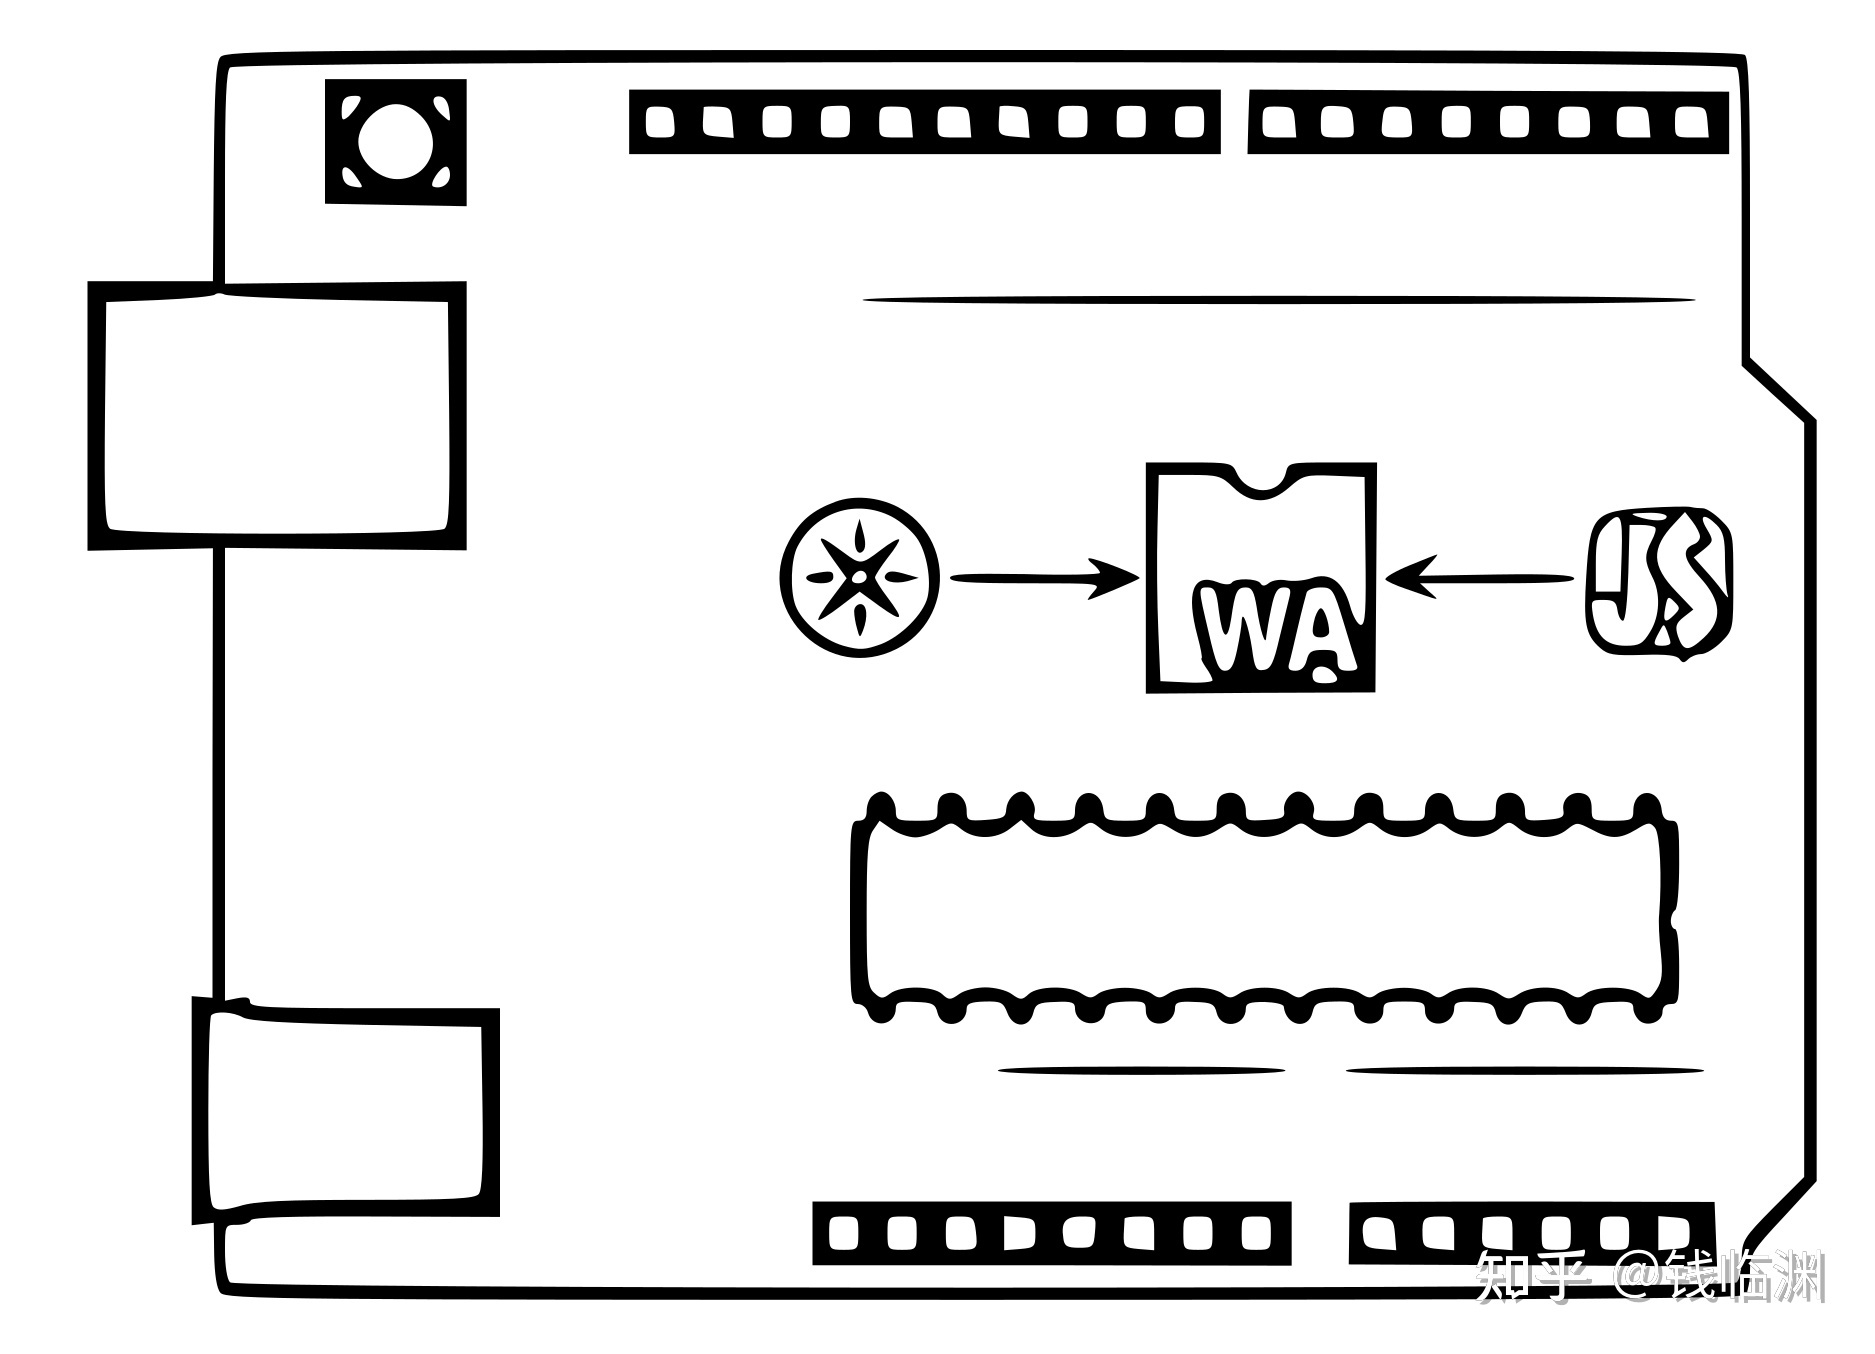
\includegraphics[width=14cm]{Chapter4/wasm.jpg}
%     \caption{WebSerialAPI+WASM}
% \end{figure}